\documentclass[aspectratio=169, 10pt]{beamer}

% ==============================================================================
% THEME & STYLING CONFIGURATION
% ==============================================================================
\usetheme{Madrid}
\usecolortheme{whale}

% Typography & Encoding
\usepackage[utf8]{inputenc}
\usepackage[T1]{fontenc}
\usepackage{lmodern}
\usepackage{microtype}

% Tables & Formatting
\usepackage{booktabs}
\usepackage{tabularx}
\usepackage{array}
\usepackage{colortbl}

% Graphics & TikZ Flowcharts
\usepackage{graphicx}
\usepackage{tikz}
\usetikzlibrary{shapes.geometric, arrows.meta, positioning, fit, calc, backgrounds}

% Custom Color Palette (Modern Biotech Theme)
\definecolor{primaryBlue}{RGB}{20, 50, 95}
\definecolor{accentTeal}{RGB}{0, 140, 150}
\definecolor{lightGray}{RGB}{245, 247, 250}
\definecolor{darkGray}{RGB}{50, 54, 58}
\definecolor{successGreen}{RGB}{34, 139, 34}
\definecolor{alertRed}{RGB}{180, 40, 40}
\definecolor{boxBg}{RGB}{238, 244, 250}
\definecolor{planBlue}{RGB}{41, 128, 185}

% Apply Color Theme to Beamer Elements
\setbeamercolor{palette primary}{bg=primaryBlue, fg=white}
\setbeamercolor{palette secondary}{bg=accentTeal, fg=white}
\setbeamercolor{palette tertiary}{bg=primaryBlue!80!black, fg=white}
\setbeamercolor{structure}{fg=primaryBlue}
\setbeamercolor{title}{bg=primaryBlue, fg=white}
\setbeamercolor{frametitle}{bg=primaryBlue, fg=white}
\setbeamercolor{block title}{bg=primaryBlue, fg=white}
\setbeamercolor{block body}{bg=boxBg, fg=darkGray}
\setbeamercolor{block title example}{bg=successGreen, fg=white}
\setbeamercolor{block body example}{bg=successGreen!8, fg=darkGray}
\setbeamercolor{block title alerted}{bg=alertRed, fg=white}
\setbeamercolor{block body alerted}{bg=alertRed!8, fg=darkGray}

\setbeamertemplate{navigation symbols}{}
\setbeamertemplate{footline}[frame number]

% Custom Itemize Spacing for Single-Line Bullets
\setbeamertemplate{itemize/enumerate body begin}{\setlength{\itemsep}{0.35cm}}
\setbeamertemplate{itemize items}[square]

% ==============================================================================
% PRESENTATION METADATA
% ==============================================================================
\title[Targeted Nanopore Epigenetic Analysis]{Targeted Genomic Region and Epigenetic Analysis Using Oxford Nanopore Sequencing}
\author[Group 17]{Vishnu - CB.SC.U4AIE23352}
\institute[DNA Sequencing Technologies]{Group Number: 17 \\[0.15cm] Course: DNA Sequencing Technologies}
\date{\today}

% ==============================================================================
% DOCUMENT BODY
% ==============================================================================
\begin{document}

% ------------------------------------------------------------------------------
% SLIDE 1: TITLE SLIDE
% ------------------------------------------------------------------------------
\begin{frame}[plain]
    \titlepage
\end{frame}

% ------------------------------------------------------------------------------
% SLIDE 2: INTRODUCTION
% ------------------------------------------------------------------------------
\begin{frame}{Introduction}
    \vspace{0.4cm}
    \begin{itemize}
        \item Oxford Nanopore enables real-time, single-molecule native DNA sequencing without read length limitations.
        \item Long reads effectively resolve complex repetitive regions, large structural variations, and homologous loci.
        \item Cas9-targeted sequencing (nCATS) selectively enriches specific genomic regions without PCR amplification.
        \item Native DNA sequencing directly detects epigenetic modifications like 5-methylcytosine ($5\text{mC}$) from ionic current.
        \item Targeted enrichment enables high sequencing depth at selected genomic loci while reducing the sequencing required compared with whole-genome analysis.
    \end{itemize}
\end{frame}

% ------------------------------------------------------------------------------
% SLIDE 3: PROBLEM STATEMENT
% ------------------------------------------------------------------------------
\begin{frame}{Problem Statement}
    \vspace{0.4cm}
    \begin{itemize}
        \item Short-read sequencing approaches face challenges in resolving complex repetitive regions, structural variations, and extended haplotypes.
        \item Standard bisulfite sequencing (WGBS) involves harsh chemical treatment that degrades template DNA and can introduce amplification biases.
        \item Whole-genome long-read sequencing remains resource-intensive when high sequencing depth is needed over specific genomic regions of interest.
        \item Asymmetric Cas9 adapter ligation produces strand-preferential read patterns, necessitating strand-aware filtering for variant validation.
        \item Downstream workflows require integrated pipelines to jointly evaluate sequence variation, phasing, and native epigenetic marks from targeted reads.
    \end{itemize}
\end{frame}

% ------------------------------------------------------------------------------
% SLIDE 4: OBJECTIVES
% ------------------------------------------------------------------------------
\begin{frame}{Objectives}
    \vspace{0.3cm}
    \begin{itemize}
        \item Perform comprehensive quality control (length, N50, Phred scores) on raw native Nanopore reads.
        \item Construct target references from GRCh38.p13 and quantify coverage across 10 selected genomic loci.
        \item Implement strand-concordant variant calling to filter false positives and identify high-confidence SNVs/indels.
        \item Reconstruct contiguous long-read haplotype phase blocks using WhatsHap.
        \item Profile native CpG methylation frequencies and validate against benchmark GM12878 WGBS data.
        \item Identify candidate structural variants within the targeted regions using long-read analysis.
    \end{itemize}
\end{frame}

% ------------------------------------------------------------------------------
% SLIDE 5: DATASET DESCRIPTION
% ------------------------------------------------------------------------------
\begin{frame}{Dataset Description}
    \begin{columns}[T]
        \begin{column}{0.46\textwidth}
            \begin{block}{Experimental \& Sequencing Overview}
                \begin{itemize}\footnotesize
                    \item \textbf{Sample:} NA12878 / GM12878 (Human Utah reference cell line)
                    \item \textbf{BioProject ID:} \texttt{PRJNA656260}
                    \item \textbf{SRA Accession:} \texttt{SRR12423814}
                    \item \textbf{Sequencing Platform:} Oxford Nanopore MinION (R9.4.1)
                    \item \textbf{Assay Method:} Cas9-targeted native DNA sequencing (nCATS)
                    \item \textbf{Reference Genome:} Human Assembly \texttt{GRCh38.p13}
                    \item \textbf{Targeted Reads Analyzed:} 23,305 reads (\texttt{SRR12423814\_1.fastq.gz})
                \end{itemize}
            \end{block}
            \vspace{-0.1cm}
            \begin{center}
                \scriptsize \textit{Native DNA sequencing preserves intact epigenetic modifications and long single-molecule fragments.}
            \end{center}
        \end{column}

        \begin{column}{0.52\textwidth}
            \begin{block}{Targeted Genomic Panel (10 Human Loci)}
                \tiny
                \begin{tabularx}{\textwidth}{l p{3.8cm} r}
                    \toprule
                    \textbf{ID} & \textbf{Associated Locus / Gene} & \textbf{Region Size} \\
                    \midrule
                    \textbf{T1} & \texttt{rs1800407} (\textit{OCA2} trait locus) & 9,886 bp \\
                    \textbf{T2} & \texttt{rs12913832} (\textit{HERC2/OCA2} regulatory) & 17,549 bp \\
                    \textbf{T3} & \texttt{rs12896399} (\textit{SLC24A4} pigmentation) & 20,355 bp \\
                    \textbf{T4} & \texttt{rs16891982} (\textit{SLC45A2} melanoma marker) & 14,845 bp \\
                    \textbf{T5} & \texttt{rs1393350} (\textit{TYR} tyrosinase gene) & 36,943 bp \\
                    \textbf{T6} & \texttt{rs12203592} (\textit{IRF4} skin phenotype) & 9,235 bp \\
                    \textbf{T7} & \texttt{TPOX} (Forensic STR Marker) & 13,778 bp \\
                    \textbf{T8} & \texttt{PentaD} (Chr 21 Pentanucleotide STR) & 16,526 bp \\
                    \textbf{T9} & \texttt{rs2814778} (\textit{ACKR1/CADM3} Duffy group) & 12,456 bp \\
                    \textbf{T10} & \texttt{rs1229984} (\textit{ADH1B} metabolic locus) & 8,252 bp \\
                    \bottomrule
                \end{tabularx}
            \end{block}
            \vspace{-0.1cm}
            \begin{center}
                \scriptsize \textcolor{successGreen}{\textbf{Panel covers key phenotypic, forensic, and metabolic regions.}}
            \end{center}
        \end{column}
    \end{columns}
\end{frame}

% ------------------------------------------------------------------------------
% SLIDE 6: PROPOSED METHODOLOGY (STANDALONE PIPELINE FLOWCHART)
% ------------------------------------------------------------------------------
\begin{frame}{Proposed Methodology: End-to-End Pipeline}
    \begin{center}
    \resizebox{0.96\textwidth}{!}{
        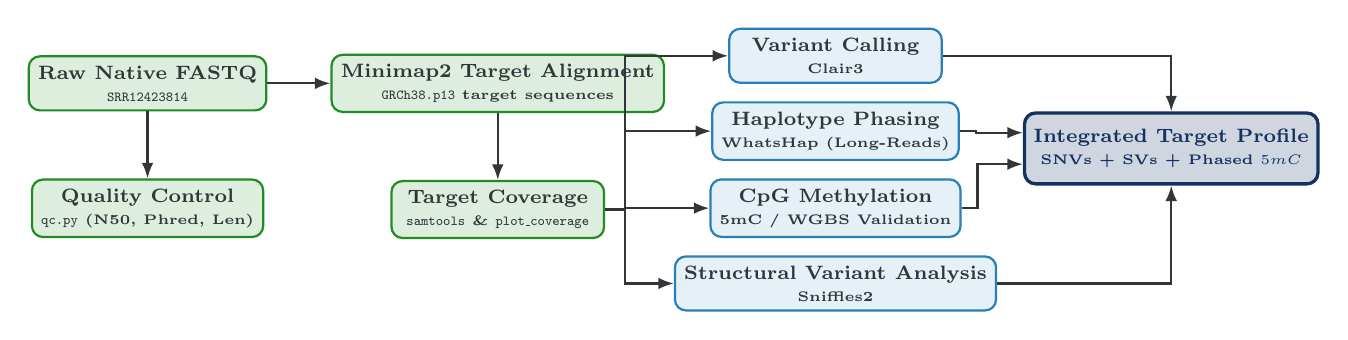
\begin{tikzpicture}[
            node distance=0.45cm and 0.65cm,
            boxDone/.style={rectangle, rounded corners=4pt, draw=successGreen, fill=successGreen!15, text=darkGray, thick, align=center, font=\scriptsize\bfseries, minimum width=2.7cm, minimum height=0.68cm},
            boxPlan/.style={rectangle, rounded corners=4pt, draw=planBlue, fill=planBlue!12, text=darkGray, thick, align=center, font=\scriptsize\bfseries, minimum width=2.7cm, minimum height=0.62cm},
            boxOut/.style={rectangle, rounded corners=4pt, draw=primaryBlue, fill=primaryBlue!20, text=primaryBlue, very thick, align=center, font=\scriptsize\bfseries, minimum width=3.0cm, minimum height=0.9cm},
            arrow/.style={-{Latex[scale=0.85]}, thick, color=darkGray}
        ]
            % Column 1: Input & QC (Completed)
            \node[boxDone] (input) {Raw Native FASTQ\\{\tiny \texttt{SRR12423814}}};
            \node[boxDone, below=0.85cm of input] (qc) {Quality Control\\{\tiny \texttt{qc.py} (N50, Phred, Len)}};

            % Column 2: Alignment & Coverage (Completed)
            \node[boxDone, right=0.8cm of input] (align) {Minimap2 Target Alignment\\{\tiny \texttt{GRCh38.p13} target sequences}};
            \node[boxDone, below=0.85cm of align] (cov) {Target Coverage\\{\tiny \texttt{samtools} \& \texttt{plot\_coverage}}};

            % Column 3: Analysis Branches (Planned)
            \node[boxPlan, right=0.8cm of align, yshift=0.35cm] (var) {Variant Calling\\{\tiny Clair3}};
            \node[boxPlan, below=0.22cm of var] (phase) {Haplotype Phasing\\{\tiny WhatsHap (Long-Reads)}};
            \node[boxPlan, below=0.22cm of phase] (meth) {CpG Methylation\\{\tiny 5mC / WGBS Validation}};
            \node[boxPlan, below=0.22cm of meth] (sv) {Structural Variant Analysis\\{\tiny Sniffles2}};

            % Column 4: Final Synthesis (Planned)
            \node[boxOut, right=0.8cm of phase, yshift=-0.22cm] (out) {Integrated Target Profile\\{\tiny SNVs + SVs + Phased $5\text{mC}$}};

            % Arrows
            \draw[arrow] (input) -- (qc);
            \draw[arrow] (input) -- (align);
            \draw[arrow] (align) -- (cov);
            \draw[arrow] (cov.east) -- ++(0.25,0) |- (var.west);
            \draw[arrow] (cov.east) -- ++(0.25,0) |- (phase.west);
            \draw[arrow] (cov.east) -- ++(0.25,0) |- (meth.west);
            \draw[arrow] (cov.east) -- ++(0.25,0) |- (sv.west);
            \draw[arrow] (var.east) -| (out.north);
            \draw[arrow] (phase.east) -- ++(0.2,0) |- ([yshift=0.2cm]out.west);
            \draw[arrow] (meth.east) -- ++(0.2,0) |- ([yshift=-0.2cm]out.west);
            \draw[arrow] (sv.east) -| (out.south);

        \end{tikzpicture}
    }
    \end{center}

    \vspace{0.1cm}
    \begin{center}
        \footnotesize
        \textcolor{successGreen}{\textbf{\rule{0.3cm}{0.3cm} Completed: QC, Alignment, Target Coverage/Depth}}
        \hspace{0.8cm}
        \textcolor{planBlue}{\textbf{\rule{0.3cm}{0.3cm} Future: Variant Calling, Phasing, Methylation, Structural Variants}}
    \end{center}
\end{frame}

% ------------------------------------------------------------------------------
% SLIDE 7: CURRENT PROGRESS: QUALITY CONTROL RESULTS
% ------------------------------------------------------------------------------
\begin{frame}{Current Progress: Quality Control Results}
    \begin{columns}[T]
        \begin{column}{0.62\textwidth}
            \begin{center}
                \textbf{\footnotesize Read Length \& Base Quality Distributions}\\[0.1cm]
                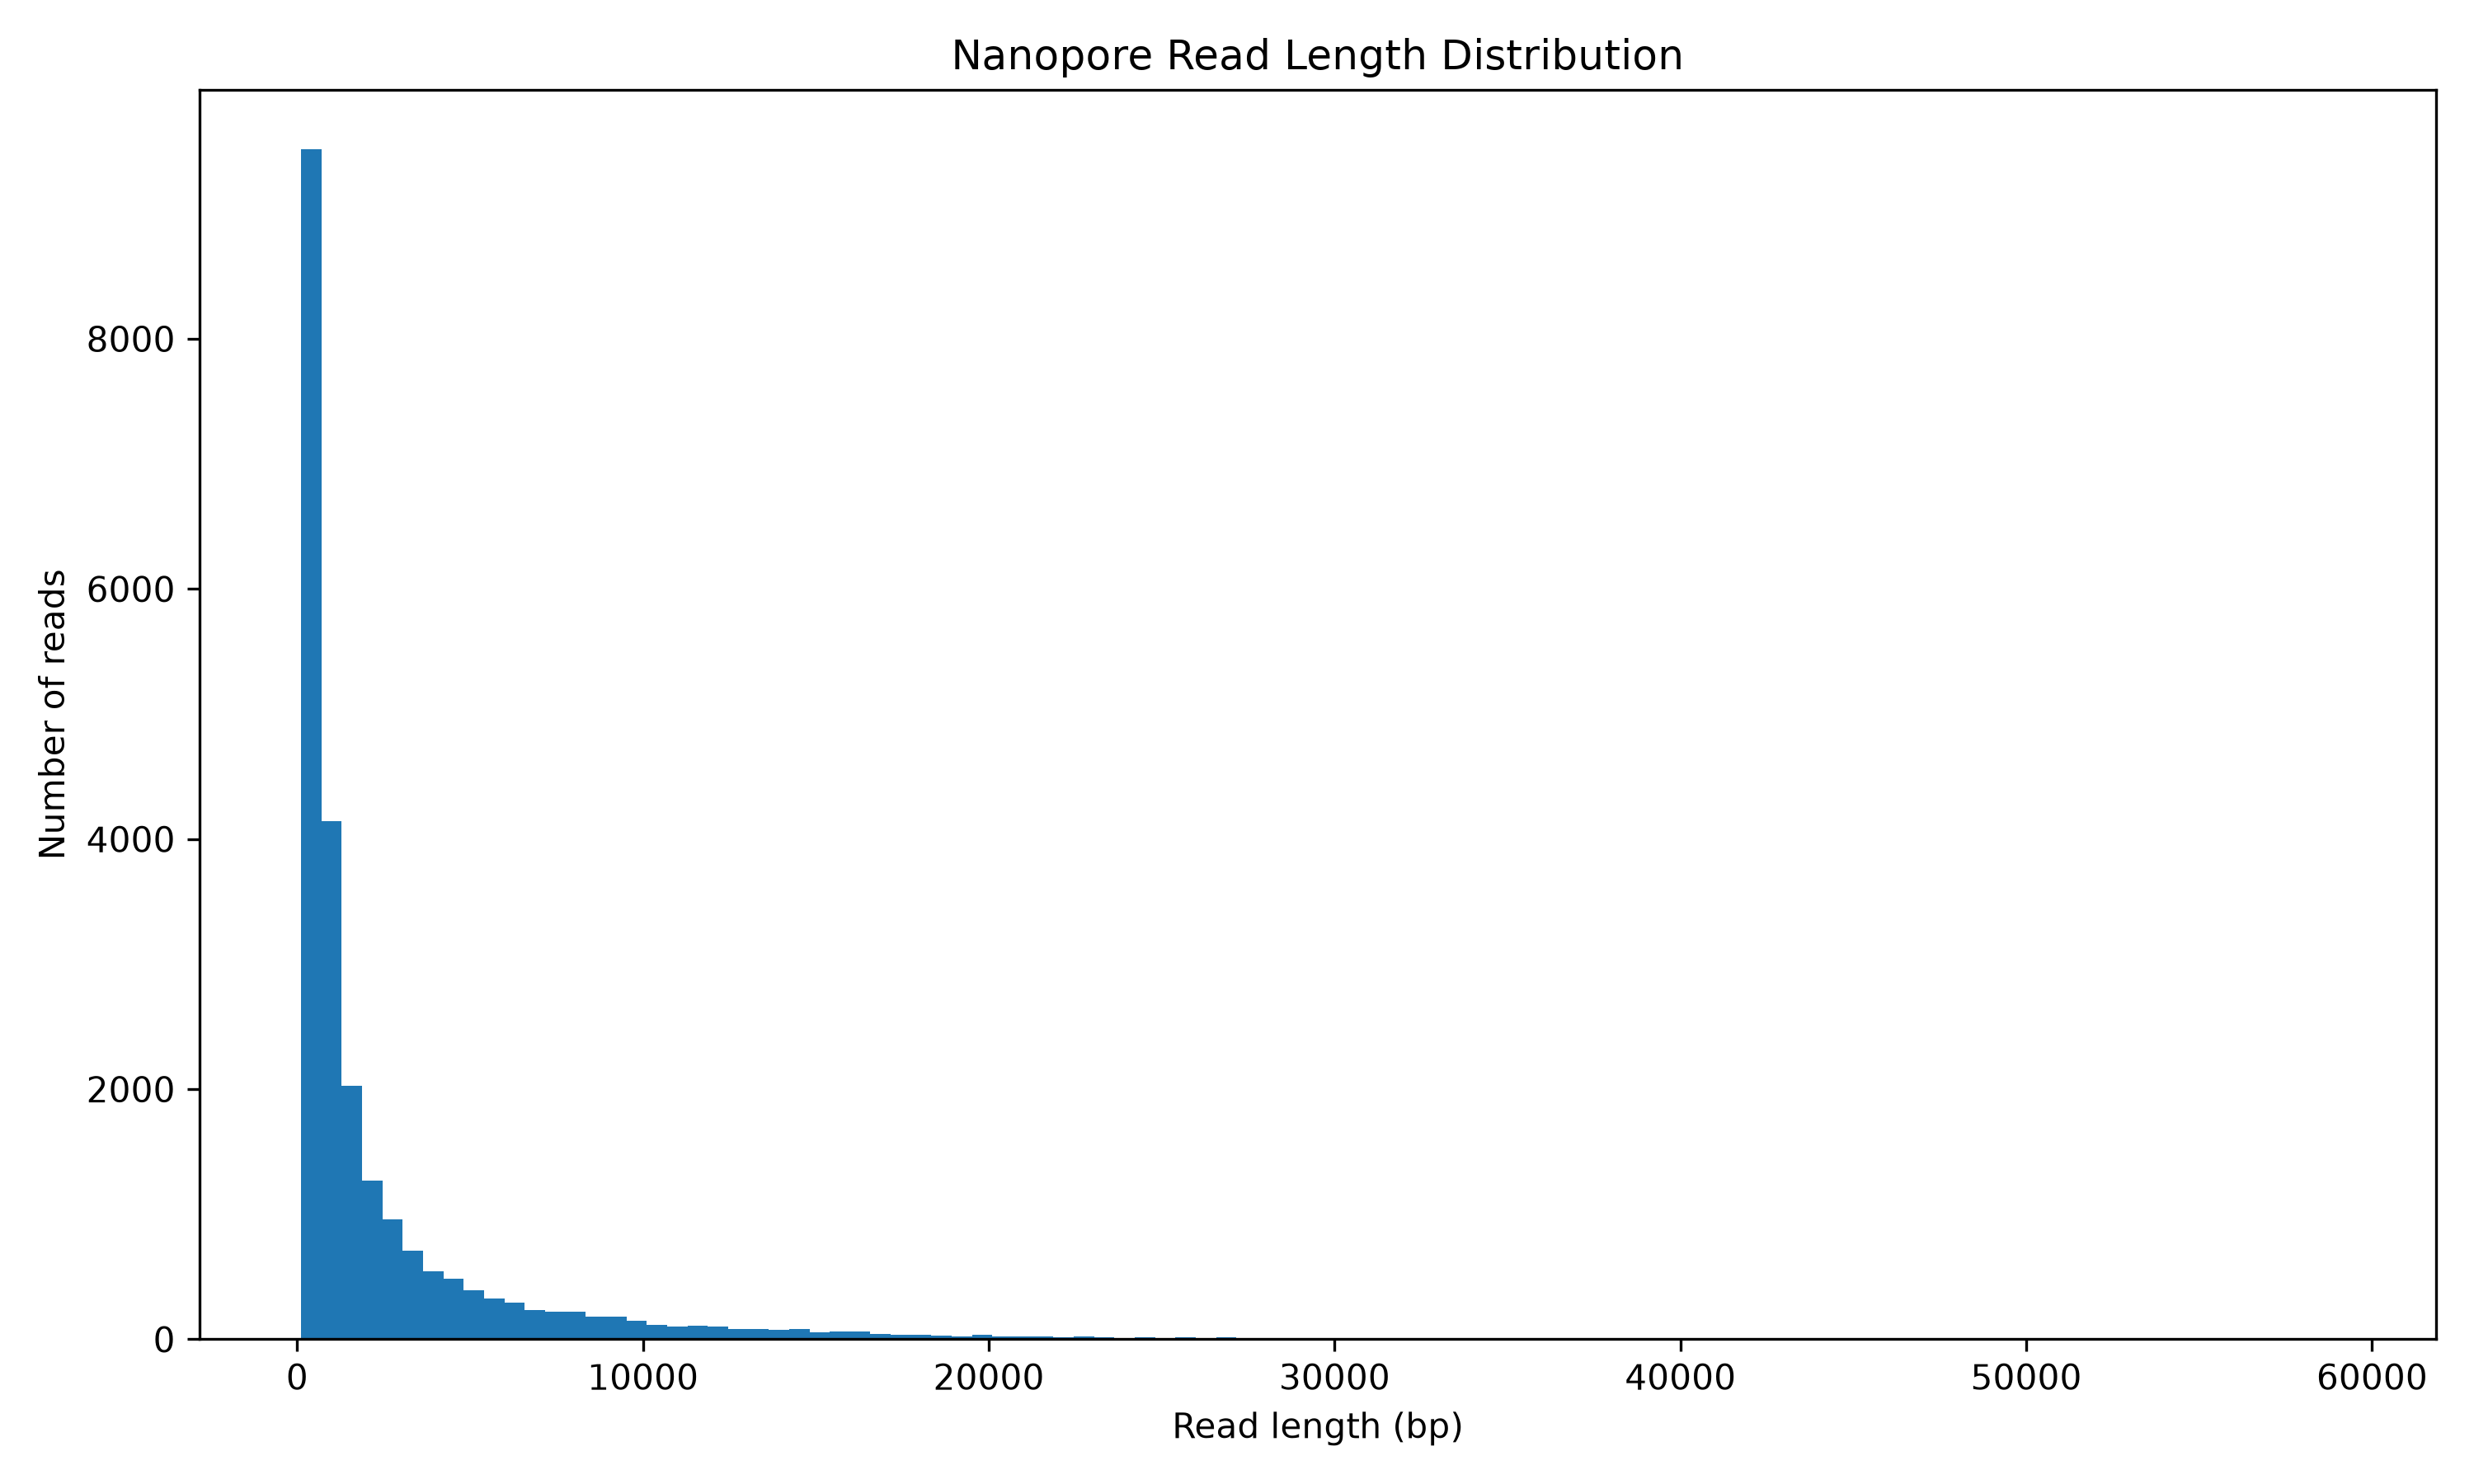
\includegraphics[width=0.48\textwidth, height=3.6cm, keepaspectratio]{read_length_distribution.png}
                \hfill
                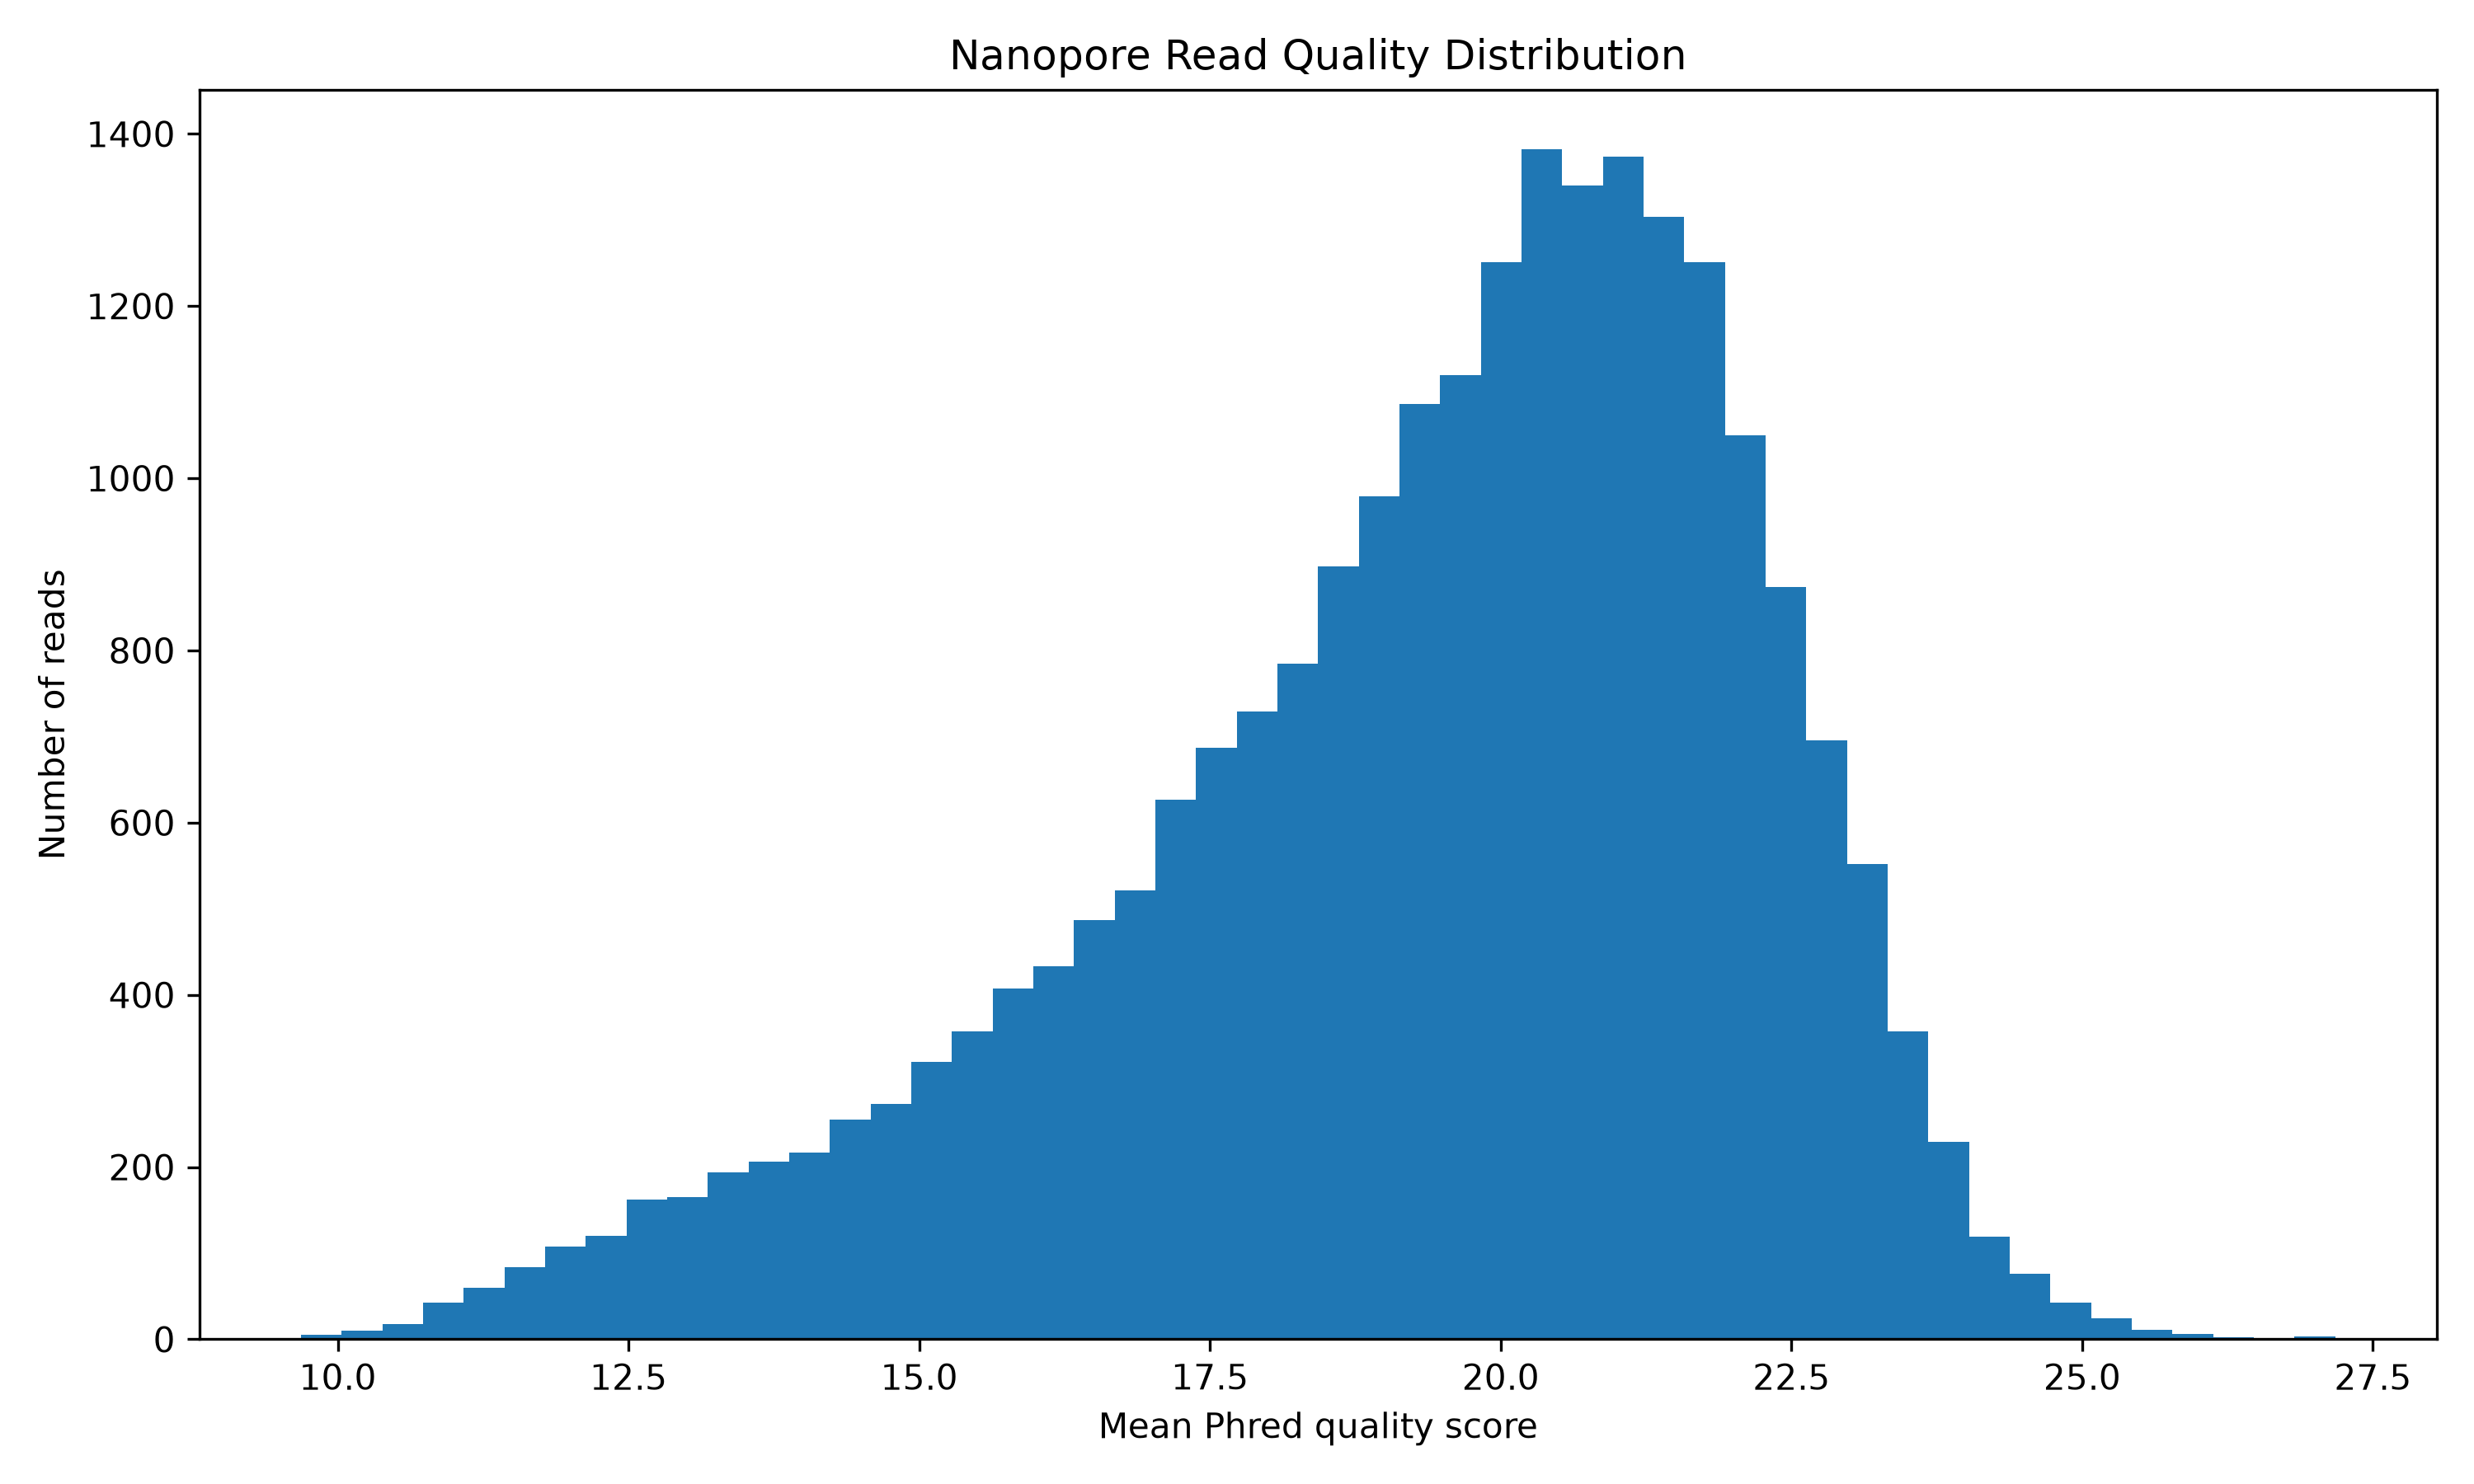
\includegraphics[width=0.48\textwidth, height=3.6cm, keepaspectratio]{quality_distribution.png}
            \end{center}
        \end{column}

        \begin{column}{0.36\textwidth}
            \begin{exampleblock}{QC Quantitative Summary}
                \begin{itemize}\footnotesize
                    \item \textbf{Total Reads Processed:} 23,305
                    \item \textbf{Total Yield:} 62,676,680 bp
                    \item \textbf{Mean Read Length:} 2,689.41 bp
                    \item \textbf{Median Read Length:} 935.00 bp
                    \item \textbf{N50 Read Length:} \textbf{7,521 bp}
                    \item \textbf{Maximum Read Length:} 58,909 bp
                    \item \textbf{Mean Phred Score:} \textbf{Q19.40}
                    \item \textbf{Median Phred Score:} \textbf{Q19.91}
                \end{itemize}
            \end{exampleblock}
            \vspace{-0.1cm}
            \begin{center}
                \scriptsize \textit{Read-quality profiles indicate that the dataset is suitable for downstream analysis.}
            \end{center}
        \end{column}
    \end{columns}
\end{frame}

% ------------------------------------------------------------------------------
% SLIDE 8: CURRENT PROGRESS: TARGET COVERAGE RESULTS
% ------------------------------------------------------------------------------
\begin{frame}{Current Progress: Target Coverage \& Depth}
    \begin{columns}[T]
        \begin{column}{0.62\textwidth}
            \begin{center}
                \textbf{\footnotesize Mean Sequencing Depth \& Coverage Breadth Across 10 Targets}\\[0.1cm]
                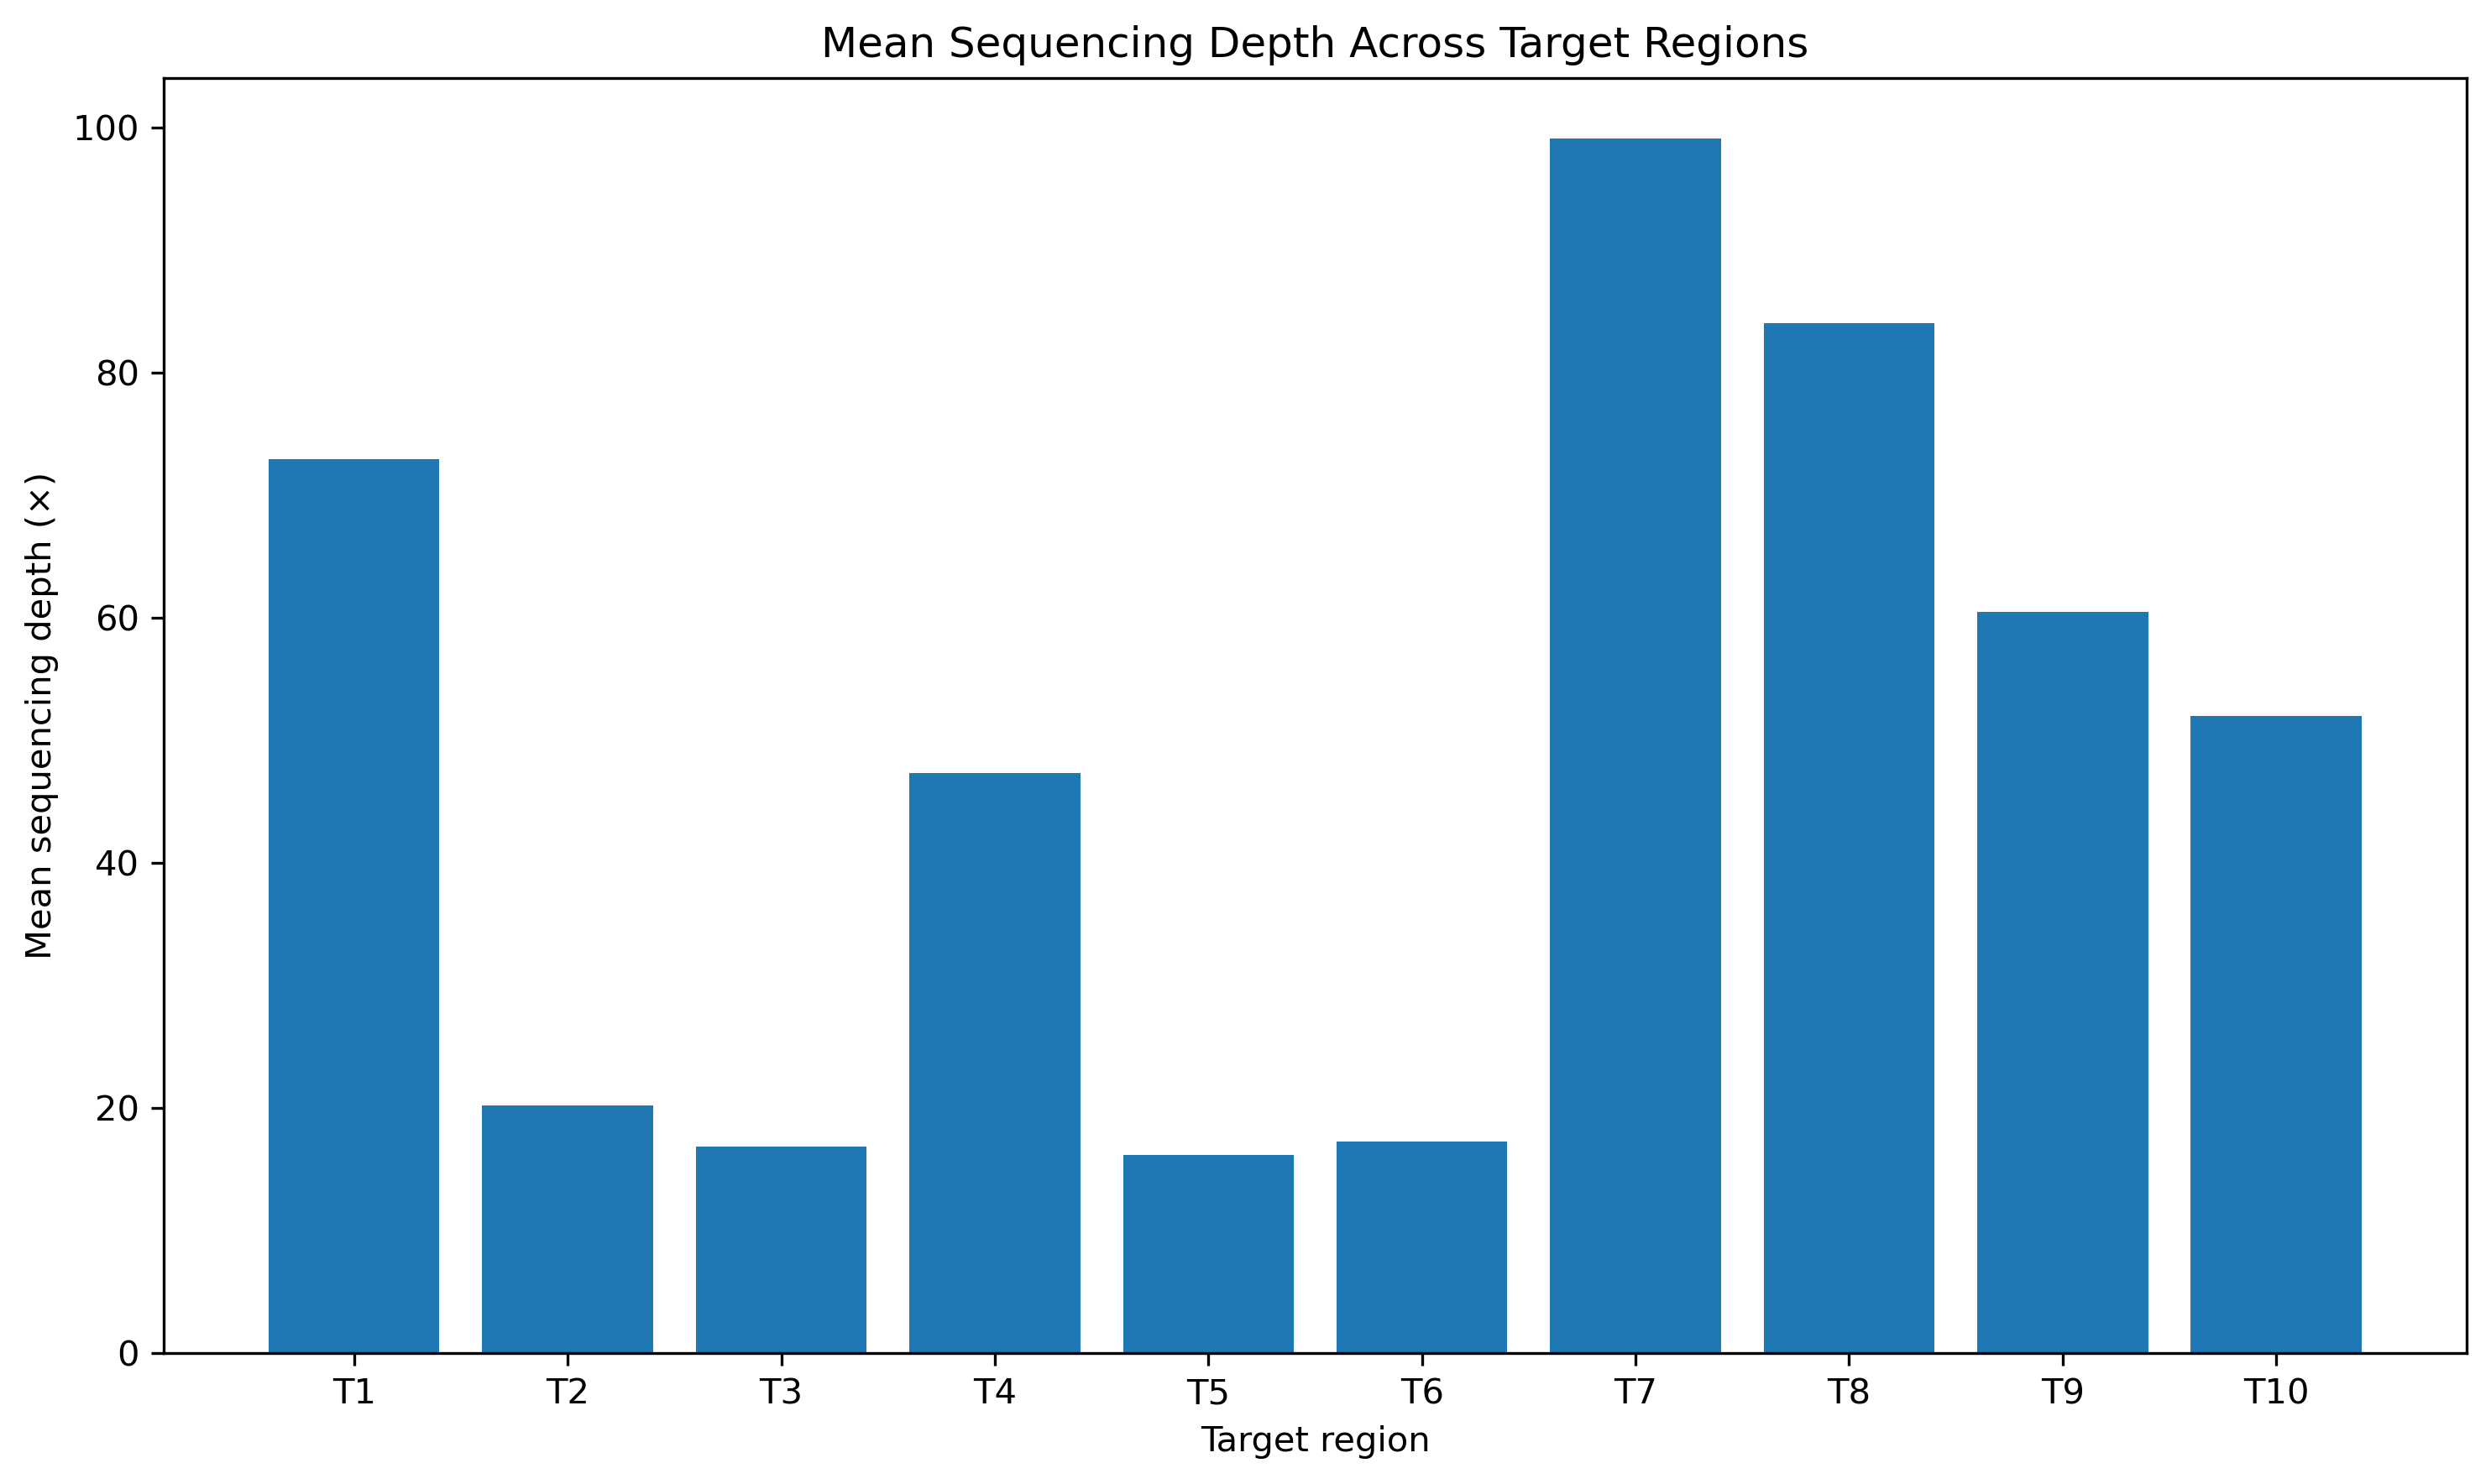
\includegraphics[width=0.48\textwidth, height=3.6cm, keepaspectratio]{mean_depth.png}
                \hfill
                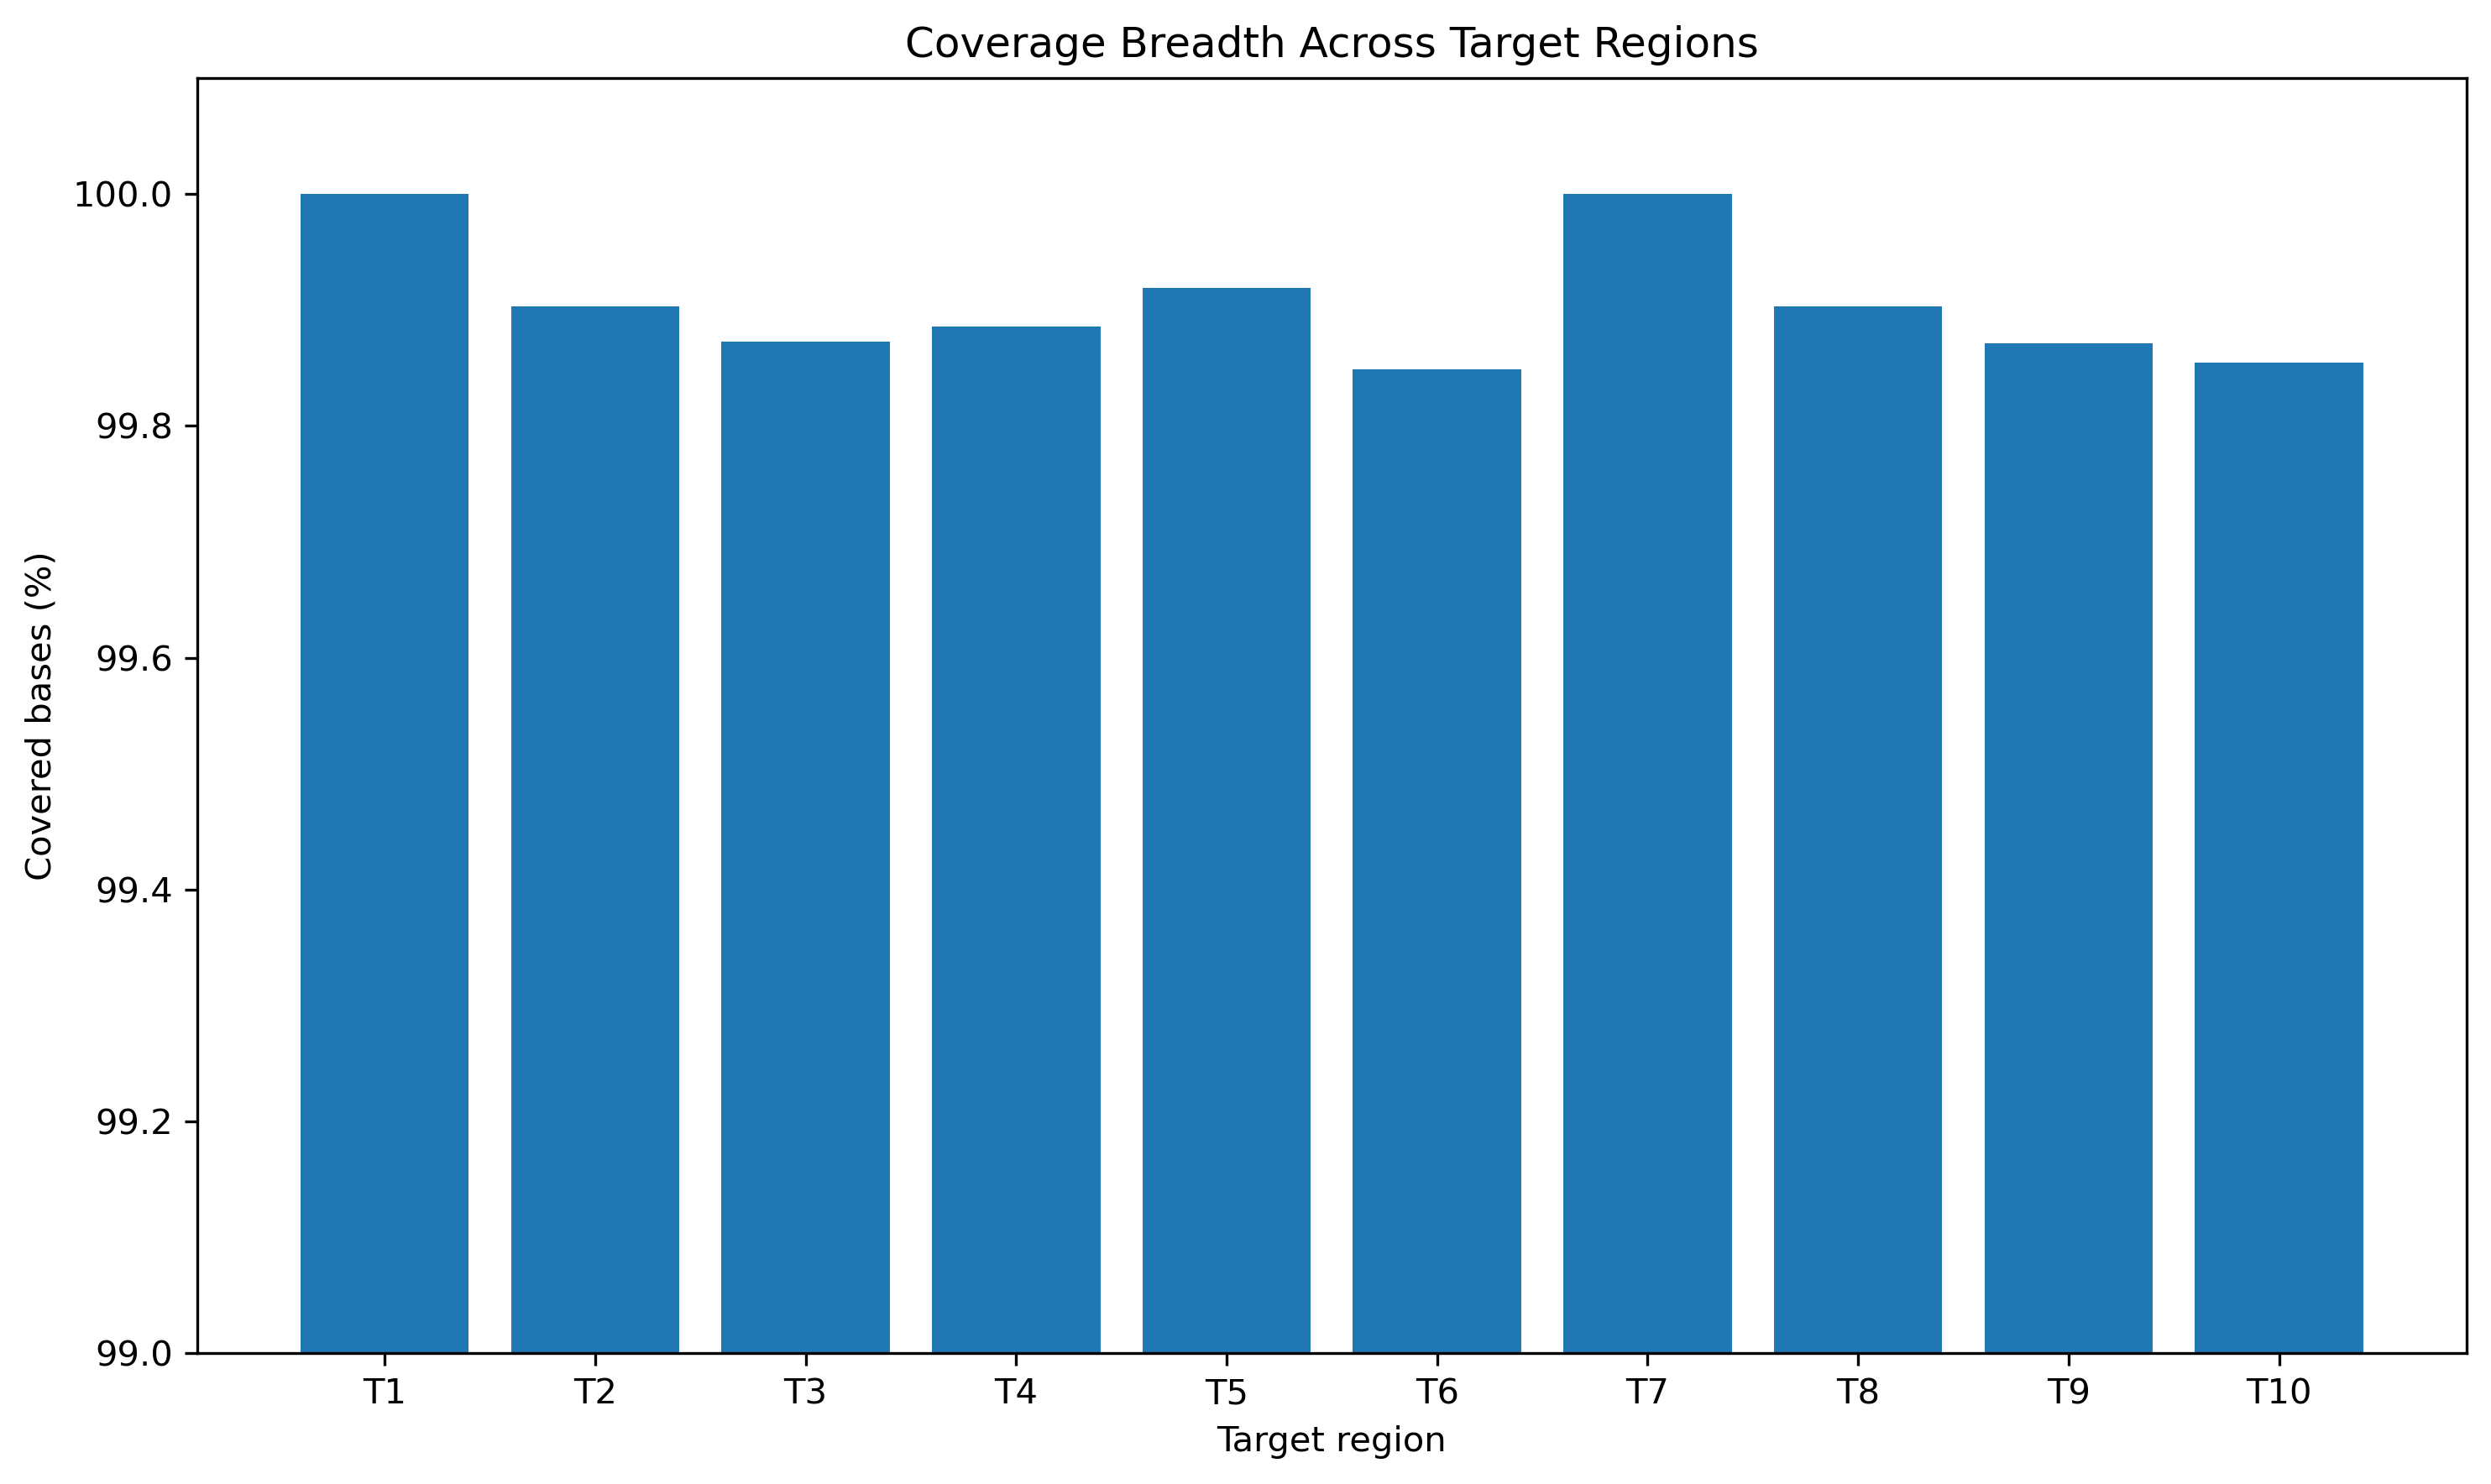
\includegraphics[width=0.48\textwidth, height=3.6cm, keepaspectratio]{coverage_breadth.png}
            \end{center}
        \end{column}

        \begin{column}{0.36\textwidth}
            \begin{exampleblock}{Coverage Key Insights}
                \begin{itemize}\footnotesize
                    \item \textbf{Coverage Breadth:} $\mathbf{>99.8\%}$ across all 10 target regions (100\% on T1 \& T7).
                    \item \textbf{Peak Depth:} Reached $\mathbf{99.09\times}$ on \texttt{TPOX} (T7) and $\mathbf{84.04\times}$ on \texttt{PentaD} (T8).
                    \item \textbf{Mean Base Q:} Ranged 19.4 to 21.5 across all target alignments.
                    \item \textbf{Target Recovery:} >99.8\% coverage breadth demonstrates consistent recovery across all 10 target intervals.
                \end{itemize}
            \end{exampleblock}
        \end{column}
    \end{columns}
\end{frame}

% ------------------------------------------------------------------------------
% SLIDE 9: KEY METHODOLOGICAL ADVANTAGES
% ------------------------------------------------------------------------------
\begin{frame}{Key Methodological Advantages}
    \begin{columns}[T]
        \begin{column}{0.48\textwidth}
            \begin{block}{Native Epigenetic Detection}
                \footnotesize
                Direct identification of 5mC modifications from Oxford Nanopore raw signal without requiring bisulfite conversion.
            \end{block}
            \vspace{0.2cm}
            \begin{block}{Dual-Strand Variant Validation}
                \footnotesize
                Planned use of strand-specific read support to reduce false-positive variant calls.
            \end{block}
        \end{column}

        \begin{column}{0.48\textwidth}
            \begin{block}{PCR-Free Target Enrichment}
                \footnotesize
                Captures native unamplified DNA molecules, preserving original base modifications and avoiding PCR-induced bias.
            \end{block}
            \vspace{0.2cm}
            \begin{block}{Multi-Feature Read Resolution}
                \footnotesize
                Enables concurrent evaluation of regional sequence variants, haplotype phase continuity, and epigenetic states from a single assay.
            \end{block}
        \end{column}
    \end{columns}
\end{frame}

% ------------------------------------------------------------------------------
% SLIDE 10: TOOLS USED IN THE PIPELINE
% ------------------------------------------------------------------------------
\begin{frame}{Tools Used in the Pipeline}
    \begin{center}
        \small
        \begin{tabularx}{0.92\textwidth}{l l p{4.5cm} l}
            \toprule
            \textbf{Pipeline Stage} & \textbf{Tool / Library} & \textbf{Function / Description} & \textbf{Current Status} \\
            \midrule
            \textbf{Quality Control} & Python 3.10 / \texttt{qc.py} & Streaming FASTQ parser, N50, Phred QC & \textcolor{successGreen}{\textbf{Completed \checkmark}} \\
            \textbf{Alignment} & \texttt{minimap2} (\texttt{map-ont}) & Long-read mapping against \texttt{GRCh38} & \textcolor{successGreen}{\textbf{Completed \checkmark}} \\
            \textbf{BAM Processing} & \texttt{samtools} 1.15+ & BAM sorting, indexing, depth extraction & \textcolor{successGreen}{\textbf{Completed \checkmark}} \\
            \textbf{Data Visualization} & \texttt{matplotlib} / \texttt{pandas} & Quantitative distribution \& bar plots & \textcolor{successGreen}{\textbf{Completed \checkmark}} \\
            \textbf{Variant Calling} & \texttt{Clair3} & Planned SNV/indel calling & \textcolor{planBlue}{\textbf{Planned}} \\
            \textbf{Haplotype Phasing} & \texttt{WhatsHap} & Read-backed long-range phasing & \textcolor{planBlue}{\textbf{Planned}} \\
            \textbf{CpG Methylation} & \texttt{modkit} / \texttt{f5c} & Native 5mC frequency quantification & \textcolor{planBlue}{\textbf{Planned}} \\
            \textbf{Structural Variants} & \texttt{Sniffles2} & Long-read structural variant discovery & \textcolor{planBlue}{\textbf{Planned}} \\
            \bottomrule
        \end{tabularx}
    \end{center}
\end{frame}

% ------------------------------------------------------------------------------
% SLIDE 11: FUTURE STEPS
% ------------------------------------------------------------------------------
\begin{frame}{Future Steps}
    \begin{columns}[T]
        \begin{column}{0.48\textwidth}
            \begin{block}{Phase 1: Strand-Aware Variant Calling}
                \begin{itemize}\footnotesize
                    \item Partition alignments by strand orientation.
                    \item Call SNVs and small indels with \texttt{Clair3}.
                    \item Filter candidate variants for dual-strand concordance.
                \end{itemize}
            \end{block}

            \begin{block}{Phase 2: Long-Read Haplotype Phasing}
                \begin{itemize}\footnotesize
                    \item Apply \texttt{WhatsHap} using long-read spanning information.
                    \item Reconstruct phase blocks across target regions.
                \end{itemize}
            \end{block}
        \end{column}

        \begin{column}{0.48\textwidth}
            \begin{block}{Phase 3: Epigenetic Profiling \& WGBS Benchmarking}
                \begin{itemize}\footnotesize
                    \item Extract per-site CpG methylation frequencies.
                    \item Evaluate correlation against reference GM12878 WGBS data.
                \end{itemize}
            \end{block}

            \begin{block}{Phase 4: Integrated Locus Characterization}
                \begin{itemize}\footnotesize
                    \item Evaluate candidate structural variants using \texttt{Sniffles2}.
                    \item Synthesize unified per-target genomic summary profiles.
                \end{itemize}
            \end{block}
        \end{column}
    \end{columns}
\end{frame}

% ------------------------------------------------------------------------------
% SLIDE 12: CONCLUSION
% ------------------------------------------------------------------------------
\begin{frame}{Conclusion}
    \vspace{0.4cm}
    \begin{itemize}
        \item Completed read-level quality control on 23,305 raw native Nanopore reads, verifying high base accuracy (mean Q19.40) and an N50 read length of 7,521 bp.
        \item Established a reference alignment workflow against GRCh38.p13 with coordinate sorting and indexing.
        \item Validated target-region coverage across all 10 genomic loci, demonstrating $>99.8\%$ coverage breadth and mean sequencing depths up to $99.09\times$.
        \item Built the foundational data processing and coverage assessment pipeline necessary for subsequent variant calling, phasing, and methylation analysis.
    \end{itemize}
\end{frame}

% ------------------------------------------------------------------------------
% SLIDE 13: THANK YOU SLIDE
% ------------------------------------------------------------------------------
\begin{frame}[plain]
    \begin{center}
        \vspace{2.2cm}
        \Huge \textbf{\textcolor{primaryBlue}{Thank You!}} \\[0.6cm]
    \end{center}
\end{frame}

\end{document}
